%-----------------------------------------------------------------------------
%
%	general.tex
%
%	AUTHOR: Ari Potkonen /JARVENPAA/ Mon Dec 11 2023
%
%	LICENSE:	All referred trademarks, logos and brand names are the
%			property of their respective owners. This document is
%			licensed under CC-BY-SA licensing scheme.
%
%			Any of the trademarks, service marks, collective
%			marks, design rights, or similar rights that are
%			mentioned, used, or cited are the property of their
%			respective owners. Their use here does not imply that
%			you may use them for any purpose other than for the
%			same or a similar informational use as contemplated by
%			the original author of document licensed under the
%			CC-BY-SA licensing scheme. Author cannot grant any
%			rights to use any otherwise protected materials. Your
%			use of any such or similar incorporeal property is at
%			your own risk.
%
%	LANGUAGE:	LaTeX2e to be used with latexmk
%
%
%	REFERENCE (http://latex-project.org/help/books http://tug.org/books):
%
%	http://ctan.org/starter
%	http://ctan.org/pkg/amsmath
%	http://ctan.org/pkg/biblatex
%
%	http://wikibooks.org/wiki/LaTeX
%	http://wikipedia.org/wiki/BibTeX
%	http://bibtex.com/format/fields
%	http://loc.gov/marc
%	http://issn.org
%
%	Michel Coossens, Frank Mittelbach, Alexander Samarin:
%	  The LaTeX Companion, Addison-Wesley Company, Inc.
%	  United States of America 1994.
%
%	Norman Walsh:
%	  Making TeX Work, O'Reilly & Associates, Inc.
%	  United States of America 1994.
%
%	http://archive.org/details/B-001-002-139
%	http://archive.org/items/B-001-002-139/Donald_Knuth_-_The_Tex_Book.pdf
%	http://ctan.org/tex-archive/systems/knuth/dist/tex/texbook.tex
%	http://visualmatheditor.equatheque.net/doc/texbook.pdf
%
%	http://www.texlive.info/CTAN/info/impatient/book.pdf
%	 /usr/share/doc/texlive-doc/plain/impatient/book.pdf
%
%	file:///usr/share/doc/texlive-doc/texlive/index.html
%	  find /usr/share/doc/*tex* -iname "*.pdf" | less
%
%	/usr/share/doc/make-doc/make.pdf.gz
%	file:///usr/share/doc/make-doc/make.html/index.html
%
%	https://ctan.org/topic/font-maths
%	https://ctan.org/tex-archive/fonts
%	https://tug.org/FontCatalogue/mathfonts.html
%
%	Edition defines major releases of document.	
%	EDITION:	0
%
%	Version defines minor changes which can be brought available online.
%	VERSION:	
%
%	CHANGED:
%	DOCUMENT HISTORY:
%
%	FUTURE:
%
%	COMPILE:	make
%			make clean
%
%-----------------------------------------------------------------------------
%        1         2         3         4         5         6         7
%23456789012345678901234567890123456789012345678901234567890123456789012345678
%-DOCUMENT PREAMBLE-----------------------------------------------------------
% /usr/share/doc/texlive-doc/latex/comprehensive/symbols-a4.pdf
\documentclass[a5paper,final]{memoir}
\usepackage[english]{babel}
\usepackage{advdate}
\usepackage{fontspec} % /usr/share/doc/texlive-doc/latex/fontspec/fontspec.pdf
\usepackage[gen]{eurosym}
\usepackage{unicode-math} % texlive-doc/latex/unicode-math/unicode-math.pdf
\usepackage{nicefrac}
\usepackage{float}
\usepackage{graphicx} % /usr/share/doc/texlive-doc/latex/graphics/graphicx.pdf
\usepackage{epsfig} % /usr/share/doc/texlive-doc/latex/graphics/epsfig.pdf
\usepackage{rotating} % /usr/share/doc/texlive-doc/latex/graphics/rotating.pdf
\usepackage{supertabular}
%\usepackage{hyphenat}
\hyphenation{
 pos-i-tron
 pos-i-trons
}
\usepackage{csquotes} % /usr/share/doc/texlive-doc/latex/csquotes/csquotes.pdf
\usepackage{biblatex}
\usepackage{xurl} % /usr/share/doc/texlive-doc/latex/xurl/xurl.pdf
\usepackage[bookmarks=true,hidelinks]{hyperref} % hyperref/hyperref-doc.pdf
\usepackage{bookmark} % /usr/share/doc/texlive-doc/latex/bookmark/bookmark.pdf
\bibliography{biblatex} %   share/doc/texlive-doc/latex/biblatex/biblatex.pdf
\usepackage{pdfpages} %/usr/share/doc/texlive-doc/latex/pdfpages/pdfpages.pdf
\usepackage{makeidx}
\setmainfont{Linux Libertine O}
\makeindex
\begin{document}
\pagenumbering{gobble}
\title{\Huge\textbf{Electromagnetism\linebreak energy and space}
\linebreak Keep It Simple Stupid\linebreak (KISS) -- Ideas \linebreak
\linebreak REPLAY \linebreak
\linebreak
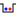
\includegraphics[height=32pt,width=32pt]{fig/ep-dwell.eps} \linebreak
\linebreak
\small
For discussions from the nature's nature !\linebreak
(http://github.com/apotkonen/gt)
}
\author{\Large Potkonen Ari}
\SetDate[25/12/2023]
\maketitle
\pagebreak
\pagestyle{plain}
\parindent 0pt
\setcounter{page}{1}
\pagenumbering{roman}
%-----------------------------------------------------------------------------
%
%	preface.tex Document preface part
%
%	INCLUDE FILE FOR LaTeX2e DOCUMENT
%
%	AUTHOR: Ari Potkonen /JARVENPAA/ Sat Dec 09 2023
%-----------------------------------------------------------------------------
%        1         2         3         4         5         6         7
%23456789012345678901234567890123456789012345678901234567890123456789012345678
%-BEGIN OF INCLUDE FILE-------------------------------------------------------
PREFACE
\label{preface}
\index{preface}
\vskip\baselineskip
\addcontentsline{toc}{chapter}{Preface}
Personally I have been missing clear coupling and simplicity between
electromagnetism and quantum mechanics modeling, which is fuzzy area,
overloaded with the terms. Peoples have done good work, and existing
models are usable for the practical life. Still there is need to go
back in time and lift again obvious possible connection between
electromagnetism and quantum physics, if there is any possibility to
get any clearance to our relativistic world. Now we use lazy mathematician
method: Guess the correct answer and let the others to proof that your and
other historic proposals were right. Here correct answer is found with the
simple "Duck test": "If it walks like a duck, looks like a duck, and quacks
like a duck, it's a duck". In practice I state that there is only
electromagnetism and space in our relativistic world, noting else, nothing
less. Electromagnetism itself is kind of progressing phenomenon, supporting
causality and offers us as humans possibility to define time which is handy
for modeling and tracking this causality, but time definition itself is
also based to electromagnetism and space, the major ingredients just
proposed for our generally relativistic world.
I really do not go to mathematic models, because then we overload ourselves
and loose our target under mass of details. I try to explain needed change
in our thinking in simplistic way, referring things we know from general
relativity, and keeping in mind electromagnetic space nonlinearity; high
field density -- bending electromagnetic space -- discrete curled wave
form -- both handed forms -- behave as mass -- energy dwell -- gravity.

Hopefully you'll get some ideas from here for your professional life!
\vskip\baselineskip
Sincerely yours Ari Potkonen
\vspace*{\fill}
%-END OF INCLUDE FILE---------------------------------------------------------

\include{rights}
\pagebreak
\tableofcontents
\listoffigures
\vspace*{\fill}
\clearpage
\pagestyle{headings}
\setcounter{page}{1}
\pagenumbering{arabic}
\parindent 0pt
%-----------------------------------------------------------------------------
%
%	story.tex Document supposition part
%
%	INCLUDE FILE FOR LaTeX2e DOCUMENT
%
%	AUTHOR: Ari Potkonen /JARVENPAA/ Mon Dec 11 2023
%-----------------------------------------------------------------------------
%        1         2         3         4         5         6         7
%23456789012345678901234567890123456789012345678901234567890123456789012345678
%-BEGIN OF INCLUDE FILE-------------------------------------------------------
\begin{comment}\end{comment}
\chapter{Guessing correct answer}
\section{Supposition}
\label{supposition}
\index{supposition}
Supposition is that our generally relativistic world we see consists only from
electromagnetism and space. % Relativistic electromagnetic space?
Nothing else is there !

Electromagnetism itself is kind of progressing phenomenon, supporting
causality and offers for humans possibility to define time, which is handy for
modeling and tracking this causality, but time definition itself is based to
electromagnetism and space, the major ingredient what just proposed for our
generally relativistic world.


\section{Hypothesis}
\label{hypothesis}
\index{hypothesis}

Hypothesis is that subatomic particles electron, positron, proton and
antiproton are actually pure electromagnetic waveforms -- curled up space.

Schwinger limit (Julian Schwinger \cite{SchwingerLimit}) gives limits for
electric field $E_c~=1.23 EV/m$ (Eksa Volt / meter) and magnetic field
$B_c~=4.41 GT$ (Giga Tesla) after we can see relativistic electromagnetic
space nonlinearity in scale of electron Compton wavelength
(Arthur Compton \cite{ComptonWavelength}) $\lambda_e=2426 fm$.


Strong electromagnetic fields in Compton wavelength scale
$(\lambda=\frac{h}{mc})$
can produce discreet numerable curled waveforms
$(\bar{\lambda}=\frac{\lambda}{2\pi})$,
$\bar{\lambda}_e=386 fm$,
%\bar{\lambda}\lambdabar\lambdaslash\textcrlambda
small discreet relativistic electromagnetic space shrinkage -- harmonic
where wave goes with light speed, but from local observers perspective outside
from curled, shrunken space, seems to be stopped and we see kind of frozen
representation from curled wave. Relativistic electromagnetic space shrinkage
represents gravity of this formed energy-dwell trapped energy.

\begin{equation} \label{eq:reduced_plank_constant} 
	\hbar
	= \frac{6.582119569}{10^{16}}[eVs]
	= \frac{1.054571817}{10^{34}}[Js]
\end{equation}

\begin{equation} \label{eq:plank_constant} % SI-units and other 
	h
	= \frac{4.135667696}{10^{15}}\left[\frac{eV}{Hz}\right]
%	= \frac{1.602176634C\cdot4.135667696V}{10^{34}Hz}
%	= \frac{1.602C\cdot4.136V}{10^{34}Hz}
	= \frac{6.62607015}{10^{34}}\left[\frac{J}{Hz}\right]
\end{equation}

\begin{equation} \label{eq:electron_rest_mass}
	m_e=\frac{E_e}{c^2}
%	=\frac{E_e [eV]}{c^2 \left[\frac{m^2}{s^2}\right]}
%	=m_e\frac{[J]}{\left[\frac{m^2}{s^2}\right]}
%	=m_e\frac{[kg\frac{m^2}{s^2}]}{\left[\frac{m^2}{s^2}\right]}
%	=m_e[kg]
\end{equation}

Electron curled spacetime radius $\bar{\lambda}_e$ is
\begin{equation} \label{eq:gamma_lenght}
%Electron annihilation induced gamma ray wavelength 
 \bar{\lambda}_e=\frac{\hbar}{m_ec}
 =\frac{\hbar c}{E_e}
 =\frac{6.58eVs\cdot299\frac{m}{s}}{10^{13}\cdot511eV}
%=\frac{6.582119569eVs\cdot299792458\frac{m}{s}}{10^{16}\cdot510998.95069eV}
 =386fm
%=386.159267407fm
%=0.386pm
\end{equation}
and diameter $\diameter_e=772 fm$.


Electron annihilation released $\gamma$ -photon wavelength $\lambda_\gamma$ is
\begin{equation} \label{eq:gamma_lenght}
% Electron annihilation induced gamma ray wavelength 
 \lambda_\gamma=\frac{h}{m_ec}
%=\lambda_\gamma\frac{\left[\frac{eV}{Hz}\right]}{[kg]\left[\frac{m}{s}\right]}
%=\lambda_\gamma\frac{[Js]}{\left[kg\frac{m}{s}\right]}
%=\lambda_\gamma\frac{\left[kg\frac{m^2}{s}\right]}{\left[kg\frac{m}{s}\right]}
%=\lambda_\gamma[m]
 =\frac{hc}{E_e}
 =\frac{4.14eVs\cdot299\frac{m}{s}}{10^{12}\cdot511eV}
%=\frac{4.135667696eVs\cdot299792458\frac{m}{s}}{10^{15}\cdot510998.95069eV}
%=2436 fm
 =2.436pm
%=2.42631023867(73)pm % https://physics.nist.gov/cgi-bin/cuu/Value?ecomwl
\end{equation}

There are few possibilities what has happened so that electron, pos\-i\-tron
could hold that electromagnetic wavelet -- $\gamma$ photon electromagnetic
energy in after pair production; Either space is bending with light speed in
curl so wave seems to be static or time, as we understand it, has been stopped
because wave in curl curving proceeds with light speed or both because light
speed is reached in formed curl. It's kind of total internal reflection
forming standing wave having only one peak visible for externals and other
peak is fully internal, only visible inside of curl. This bending makes curled
wave behave like noticeable charged particle, still being a discreet standing
wave due to nonlinearity making it possible to exist.

Curling can create discreet numbered relativistic bending forms to space, and
we call known stable curl forms to electron, positron, proton and antiproton.

Each curl's bend space around and bending is called to gravity. Bending
strength is related into curl trapped energy. Curl is kind of energy dwell
holding energy, bending and shrinking space according to trapped energy
amount. Known lowest energy curls are electron and positron. Electron curl
outside visible electric field is negative and other handed antiparticle
positron has positive electric towards outside.

Because of this outside bended electric field, local observer can accelerate,
move electrons and positrons using external electromagnetic field. When
electron, it's curl is accelerated with the external electric field it will
face relativistic Doppler effect, it's wave is coming shorter which means that
curled wave gains more energy and more mass. While decelerated curl wavelength
widens and energy is lost to breaking against the external field.

Proton and antiproton next energy rich left and right hand sided
electromagnetic field stable curls we know. Proton has positive field outwards
and antiproton has negative field outwards. While energy is much bigger than
electron has, the wavelength of curl is shorter and curl size is smaller.
Tight curl forms stronger bend to space and we see it as stronger gravity.
This bend is still kind of energy dwell. Due strong local fluctuation on
relativistic electromagnetic space, electromagnetic space itself is lead to
forming relativistic curl trapping this energy in. Forming an energy dwell
trapping energy and bending space relatively due this trapped energy.

In other words shrinkage in relativistic electromagnetic space is lower energy
state of electromagnetic space, where bending strength -- gravity as we know
represents energy dwell size as well amount of energy trapped into this dwell.

Electron negative electric field and proton positive electric field pull curls
towards each other and those can superposition over the each other still
maintaining own separate curls, proton smaller and electron bigger. This one
proton and one electron superpositioning is known as "Hydrogen-1 (protium)".

When curl and it's inverse, antimatter curl, meet happens
annihilation\allowbreak\cite{ Annihilation} where curls open, space bending
shrinkage opens -- gravity vanish and energy is again in electromagnetic form
on local space. Pair production\allowbreak\cite{PairProduction} can happen
again from this released energy.

\section{So called "weak interaction"}
\label{weak_interaction}
\index{weak interaction}

With the additional energy electron-curl
$2426$\allowbreak$fm$\allowbreak\cite{ComptonWavelength} can reach
pro\-ton-curl size $1.321$\allowbreak$fm$ and form new harmonic curl called
neutron $1.319$\allowbreak$fm$. Due to needed extra energy neutron curl, even
it's electric fields sum outside seem to be zero, is affected by external
electric disturbances and cause neutron curl decay to proton and electron
curl, average time to decay is about fifteen minutes.

This decay is called to beta $\beta$-decay to and acting force is called to
weak force. Forces come during curl creation from electron Compton wavelength
shortening taken energy -- during size shrinking for electric field
strengthening done work, and proton positive, electron negative electric
fields mutual pulling force done work. These forces and work amounts are
opposite ones, partially cancel each other, causing sum force to look a like
"weak force" or "weak interaction". Interaction begin and end state energy
levels we can see from known rest masses which directly relate to each
separate or created harmonic curl energy at rest.

\section{So called "strong interaction"}
\label{strong_interaction}
\index{strong interaction}

There is no strong interaction at all, seen strong interaction is
relativistic electromagnetic interaction. For example proton - proton
interaction is two different proton curls interaction, electromagnetic force
pulls those away from each other starting from long distances. While curls
come near by each other starting to form common harmonic curl, common
relativistic space where both electromagnetic waves fly at light speed, and
outside observer sees static view from curl having positive electric field
towards outside observer. In this case repelling forces are so big that
formed harmonic curl "Helium-2 (diproton)" isn't stable, and protons are
immediately diverging apart.

If we combine above in weak interaction told proton and electron combination
called neutron with the proton we will get the stable "Hydrogen-2
(deuterium)" harmonic curl having one positive electric field towards outside
observer, which easily form superposition with the additional electron curl.

Created harmonic curl has rest mass different from the ingredients rest masses
and that is the needed or given energy during harmonic stable curl creation or
it's breaking, those are the strong forces at common harmonic curl -- atom
core creation and breakage.

We should not use human defined term time here at all because in the curl
where field strength is so high that nonlinearity exists and affects to
electromagnetic fields, forming space curling -- shrinkage and related
gravity. Electromagnetic forces reactions in nuclear scale can be defined just
by comparing the ingredients and results rest masses. Differences are
creating the dynamic forces driven reactive movements on reaction.

Because peoples are so keen to use they time definition to understand
reactions we could give explanation using term time, so it might be helpful
when reaching the matter how strong nuclear force could be just
electromagnetic force and nothing else; When these separate waves are reaching
near by, and they both are on nearby light speed in they own curls, coming
together enough to form common curl they propagate at light speed, which means
that relativistic electromagnetic force average affecting time, impulse time,
shorter than what static observer can see, ... and understand ;-), therefore
observer sees "strong interaction" because momentum is force multiplied with
time, and now time goes slower, reaching it's relativistic way
137\allowbreak\cite{FineStructureConst} times shorter time step during
electromagnetic interaction than what observer thinks. This leads to situation
where force has to be 137 times stronger than static local observer thinks to
get if same electromagnetic effect happen in he's local reference frame. Users
reference frame where curled space internal time
dilatation\allowbreak\cite{TimeDilation} is not seen.

And if change work get done, then later on uncurling also give that same bang
backwards. Yep it's strong, but it's still electromagnetic force now forced
to happen to item going with light speed at start state in it's own curl.

This same process affects to all known more or less stable
nuclides\allowbreak\cite{Nuclides}. External conditions may wary, causing
smaller or bigger probability for certain combinations forming.

\begin{equation} \label{eq:clock_rate} % Lorentz factor
 \frac{1}{\gamma}=\sqrt{1-\frac{v^2}{c^2}}~~;~~\gamma=137.035999084
%137.035999177
\end{equation}

%\begin{equation} \label{eq:speed_rate}
%	\beta= \frac{v}{c}= \sqrt{1-\frac{1}{\gamma^2}}
%\end{equation}

%\begin{equation} \label{eq:speed_ratio}
%	\beta= \frac{v}{c}= \sqrt{1-\frac{1}{137^2}}= 0.99997
%\end{equation}

%\begin{equation}
%	\frac{v^2}{c^2}= 1-\frac{1}{\gamma^2}
%%	= n^{-2}
%\end{equation}

\begin{equation} \label{eq:speed}
	\frac{v}{c}=\sqrt{1-\frac{1}{\gamma^2}} ~=~ 0.99997
\end{equation}

%\begin{equation} \label{eq:reflective_ratio}
%	n^{-2}= \frac{\gamma^2-1}{\gamma^2}
%\end{equation}

%\begin{equation} \label{eq:reflective_ratio}
%%	n=
%	\frac{c}{v}=
%	\sqrt{\frac{\gamma^2}{\gamma^2-1}}=
%	1.000026627
%\end{equation}

%\begin{equation} \label{eq:refractive_index}
%	n= \frac{c}{v}= 1.000026627
%\end{equation}

Critical angle based to fine structure constant.

\begin{equation} \label{eq:critical_angle}
	\theta_c= \arcsin(\frac{v}{c}) = 1.5631~rad~89.556~deg
\end{equation}

%\begin{equation} \label{eq:critical_reflection_angle}
%	\theta_c= \arccos(\frac{v}{c}) = 0.0077~rad~0.4438~deg
%\end{equation}

By counting from speed difference how many internal reflections $Nr_{min}$
are needed to cover full circle $2\pi~rad = 360~deg$ we notice that about
406 reflections do the thing; Wave full internal reflection from minimum
matter amount, one electron itself.

\begin{equation} \label{eq:minimum_number_of_reflections}
	Nr_{min}\geq
	\frac {2\pi}{2\arccos(\frac{v}{c})}
	=\frac {\pi}{\arccos(\frac{v}{c})}
	= 405.58
\end{equation}

This gives kind of hint what we are looking for. Truth is some kind of limit
because formed electron or positron does not be full reflection instead it's
showing either negative or positive electric field outwards, but not both.
Kind of dot sized local space rotating so fast that light speed propagating
wave from external observers perspective seems to stay still without energy
loss or gain.

\section{Superpositioning}
\label{superpositioning}
\index{superpositioning}

Formed common curl -- atom core -- has positive electric field visible outside
and it attracts electron curls to superpositioned position balancing electric
fields. Superpositioned electrons are relatively loosely connected and related
to chemical properties of atom having core curl and superpositioned electrons.

Antimatter core curl have negative electric field visible outside and it
attracts positron curls to superpositioned position balancing electric fields
towards the outside local observer.

\section{Tunneling}
\label{tunneling}
\index{tunneling}

We do not live in isolation. Electromagnetic radiation in different waveforms,
curls, harmonic curls, superpositioned curls and excitation levels in any
local coordinate system having any speed level is still under radiation
starting from thermal radiation towards high energy cosmic rays.

Electromagnetic waves can be summed up to sum wave and this holds over the
space including the formed curls, harmonic curls and they excitation levels.
Therefore some curls forming the barrier and others being trapped in can sum
up with the external wave weakening barrier or strengthening the trapped curl
so that summed curl can pass the barrier curls formed barrier.

\section{Nuclear reactions}
\label{nuclear_reaction}
\index{nuclear reaction}

Radioactive decay is statistical value for the different curls, harmonic sum
curls aka nucleus lifetime in the local reference frame under background
radiation condition and referred matter bulk own internal statistical state.

When there is external disturbance, background radiation and surrounding curls
own curvature "gravity" and possible reaction pressure is affecting we see
different reactions, changes to harmonic sum curls listed in nuclide
chart\allowbreak\cite{Nuclides}, changes between the more or less stable
harmonic waveforms in referred background environment.

Certain bulk matter combinations can introduce chain reactions where initial
curl breakage could introduce sub curls extraction and cause more curls to
break in chain reaction aka fission.

Gravity and reaction pressure can also introduce and maintain existing curls
merge or fusion to bigger harmonic curls in chain reaction way. Reactions can
be exothermic releasing radiation, kinetic energy and straightening space or
endothermic by storing energy to created curl and creation of even more bend
electromagnetic space.

These defined reactions are reactions under one handed matter bulks. Meaning
other handed antimatter curls involvement to reactions is negligible.

\section{Great Void}
\label{great_void}
\index{great void}

One explanation to great void formation in to space is that it's original
empty undistracted space, which is not yet bended much. This partly because
creating of curls, energy dwells with trapped energy in, needs that there are
significantly high eletromagnetic fields available, meaning that there is need
to have some matter in nearby to create more matter by bending space and
trapping energy in to form energy dwells bending space and drag more matter
together. Matter which basically has got energy from more and more bending
space forming electromagnetic curl kind of energy dwell trapping energy in.

Other explanation for great void is an gigantic antimatter mass passage
through space, causing matter annihilation. Interesting thing is could this
passage formation be dated somehow, and does it have any relation to original
big bang?

\section{Big Bang}
\label{big_bang}
\index{big bang}

Material production is shown mostly be pair production creating 50\% matter
and another 50\% of antimatter. Annihilation process repeats several times
before local matter and antimatter cumulation can occur. Withing formed local
cumulations, probability that matter can stay longer intact grows. There will
be places having more matter and other places having more antimatter. This way
matter probability to survive longer grows. Any asymmetry in creation or decay
will boost cumulation significantly because there is no need to have huge
distances between before massive cumulations can occur without risk to sudden
annihilation due gravity merged local matter and antimatter cumulations
collision.

The lack of notifications from antimatter galaxies we could start to think
that does there be matter and antimatter black holes, holes maintaining the
separation of the bulk matter and bulk antimatter. Are we possibly living
in one of these black holes.

Due to expected amount of energy and mass of big bang ingredients must had,
we could say that black holes are in some amount reversible or recursive.
Because you can't have that amount mass, localized energy, without black hole
formation before bang.

Most obvious explanation for the big bang is supermassive antimatter and
matter back holes collision and expansion in combined black hole or expansion
outside of combined black hole due the matter annihilation in big way, same
time opening each particle curl which remove gravity and electromagnetic
radiation pressure overcome reduced gravity even pair production try to
maintain it, in these circumstances immediate annihilation occur and radiation
energy is free to enlarge space or even escape from black hole in form of big
bang.

Other explanation is that matter and antimatter black holes merged by
exploding black hole internal structure we are part of. This leads to
fractal structure of space.


\section{Enlarging Space}
\label{enlargind_space}
\index{enlarging space}

Due to telescopes noticed far reaching stars spectrum redshift, space is
expected to enlarge. Idea is that space is enlarging and enlargement speed
is expected to be the reason for the redshift. It's good to ask that does
this "enlarging balloon" be fully correct interpretation and what part does
gravity and space curvature play in this relative world. 

As we live in relative space where we could have different observation points
the local observer understanding may differ from the others. While thinking
massive bodies as summed energy dwells causing space to shrink the question
is that which amount of redshift is just change due light follows
brachistochrone curve or geodesic while coordinate system is same
time moving towards the energy dwell center.

If we do assumption that untouched neutral space is linear and pair
production created curvature get it shrink creating gravity as we understand
this shrinkage. Then we could tie local observers to several places on
coordinates along straight path from great void to small star, after small
star, just before giant black hole and into giant black hole.

\begin{figure}
 \begin{center}
  \epsfig{figure=fig/starhole.eps,width=\textwidth}
  \caption{Space, Star and Black Hole Energy Dwell}
  \label{fig:StarBlackHole}
 \end{center}
\end{figure}

Truth in our relative electromagnetic space might be much simpler than what
expected. It is widely accepted that electromagnetic space is nonlinear. On
event horizon space bends or shrinks so fast the light can't be escaping from
black hole, and shrinkage speed can be even more below event horizon.

So we could expect that light speed is constant as we have understood and
relativistic space shrinkage speed can overcome light speed so that light
can't escape, for example from the black hole singularity behind event
horizont.

Shortly we can summarize that light speed is constant "$c$" and space
shrinkage can be zero and as well it can overcome light speed. So space
shrinkage is independent from light speed and can overcome light speed.

Next we could turn in our space so that some great attractor, like black
hole is behind us and we are looking distant star having redshift in it's
spectrum.

Star is radiating with large scale, but normally we follow hydrogen spectral
lines deviation from the initial values.

With above expectations light from distant star leaving the star corona with
the light speed "$c$" same time as space shrinkage at star place towards
black hole is "moving coordinates" towards black hole prolonging wavelength
in electromagnetic space pointing towards us causing part of seen redshift.

Behind the star same effect cause blueshift for the light emitted away from
us, but we can't see it because it's directed outwards and behind the star.

To really have escaping star on enlarging space the cosmological redshift
"hubble constant" has to be bigger that what the "gravitational redshift".
Gravity is causing shrinking space which the looks redshift on escaping
star light.

\section{Dark Matter}
\label{dark_matter}
\index{dark matter}

Space might be fractal having space and black holes in black holes, then
average density can be higher in inner space than what local observer can
notice in near by environment, or there are unknown, unnoticed curl forms
not affecting nor reacting with the known forms.


\section{Accelerator physics}
\label{accelerator_physics}
\index{accelerator physics}

High energy accelerator physics has filled gaps from Live Chart of Nuclides
\cite{Nuclides}, given lot of Feynmann diagrams\allowbreak\cite{
FeynmannDiagram}.

%\section{Energy density}
%\label{energy_density}
%\index{energy density}
%Each gram of matter corresponds 90 TJ or 25 GWh of energy.
%\begin{equation} \label{eq:EisMc2} 
% \frac{E}{m} = c^2 = 299792458^2 \frac{m^2}{s^2} =
% 90\frac{PJ}{kg}=25\frac{GWh}{g}
%\end{equation}
%Using 1kg/s is giving more than the whole human race energy consumption.
%It's enough to use $365d/y\cdot24h/d\cdot1kg/h=8760kg/y$ to cover all
%humans energy consumption needs for whole year.
%% Electric car 18kWh/100km
%% Diesel&Petrol 46MJ/kg 12.8kWh/kg Car 5kg/100km = 64kWh/100km
%% 64kWh/100km = 2.56 mikrogram of matter /100km
%% 64kWh/100km = 1.28 mikrogram of antimatter/100km

\begin{comment}\end{comment}
%-END OF INCLUDE FILE---------------------------------------------------------

\include{formulat}
\include{proof}
%\cleardoublepage
\addcontentsline{toc}{chapter}{Bibliography}
\printbibliography[title=Bibliography, heading=bibintoc]
\addcontentsline{toc}{chapter}{Abstract}
\include{abstract}
\end{document}
\endinput
